%!TEX root = main-ugly.tex
Robust control explicitly accounts for the unavoidable mismatch between the predictions made by a mathematical model of a system, and the behavior of the system itself.  In the context of linear control systems, robust control techniques \cite{khammash1990stability,dahleh1994control,zhou1996robust} have proven invaluable in applications ranging from process control to aerospace engineering.  A challenge in robust control is the tension between how detailed a description of model uncertainty is available, and the conservativeness of corresponding computationally tractable analysis and synthesis tools.  Indeed, many of the celebrated tools from robust control, such as the structured singular value (see \cite{packard1993complex}), structured small gain theorems (see Ch 7.2 of \cite{dahleh1994control}), and integral quadratic constraints (IQCs) (see \cite{megretski1997system}), seek to optimally navigate this tension.  However, as of yet, few of these results have been extended in a provably non-conservative manner to the large-scale distributed setting.

Although there is a rich and increasingly mature body of work tackling the distributed optimal control of linear systems (see \cite{2006_Rotkowitz_QI_TAC, 2012_Mahajan_Info_survey, wang2019system,zheng2019equivalence}, and references therein), some of which have robust stability interpretations with respect to unstructured norm bounded uncertainty (e.g., \cite{langbort2004distributed,matni2014distributed,lessard2014state,rosinger2017structured,ahmadi2018distributed}), to the best of our knowledge no necessary and sufficient conditions for the robust performance of large-scale distributed controllers exist.  Another branch of related work are methods that use dissipativity theory combined with distributed optimization techniques to derive sufficient conditions for the stability of known interconnected systems, see for example \cite{arcak2016networks,meissen2015compositional,anderson2011dynamical} and the references therein -- while applicable to large-scale systems, these methods can be conservative.

In this paper, we address this gap by leveraging the System Level Synthesis (SLS)  framework \cite{anderson2019system,wang2019system}.  SLS reformulates robust and optimal control problems as an optimization over the achievable closed loop behavior, or \emph{system responses}, of a linear-time-invariant (LTI) dynamical system, and in particular shows that it is necessary and sufficient to constrain these system responses to lie in an affine subspace defined by the dynamics.  This parameterization has been successfully exploited in the context of the distributed optimal control of finite-dimensional LTI systems to scale controller synthesis and implementation techniques to systems of arbitrary size under practically realistic assumptions on the underlying system \cite{wang2014localized, wang2016localized,wang2018separable}.  

In order to accommodate general linear time varying uncertainty, we extend the SLS parameterization of internally stabilizing controllers to a class of systems described by causal bounded linear operators, and show how this parameterization can be used to make connections to $\mathcal{L}_1$ robust synthesis techniques \cite{khammash1990stability,dahleh1994control}.  In doing so, we derive necessary and sufficient conditions for robust performance in terms of \emph{convex} constraints on the system response variables.  We then exploit this connection to show that these necessary and sufficient conditions are equally applicable when additional delay, sparsity, and locality constraints are imposed on the system responses and controller implementation.  To the best of our knowledge, these are the first such necessary and sufficient conditions for robust performance that can be verified at scale, and that produce a distributed controller with a corresponding scalable and distributed realization, making these results and their corresponding computational tools naturally applicable to large-scale uncertain systems.  In particular, our contributions are:
\begin{itemize}[leftmargin=*]
\item A generalization of the SLS parameterization of stabilizing state-feedback controllers for finite-dimensional LTI systems \cite{wang2019system} to systems with dynamics described by bounded and causal linear operators, wherein we show that constraining system responses to lie in an affine subspace defined by the system dynamics is necessary and sufficient for them to be achievable by a causal linear controller;
\item A generalization of the robustness result of \cite{matni2017scalable} showing that the  generalized SLS parameterization is stable with respect to perturbations away from the aforementioned achievability subspace, as well as an explicit characterization of the effects of these perturbations on the actual closed loop behavior achieved by the correspondingly perturbed controller implementation;
\item The formulation and solution of a robust performance problem in terms of system response variables for a linear-time-invariant dynamical system subject to bounded and causal linear uncertainty that naturally allows for delay, sparsity, and locality structure to be imposed on the system response and corresponding controller implementation;
\end{itemize}

\begin{figure}
\centering
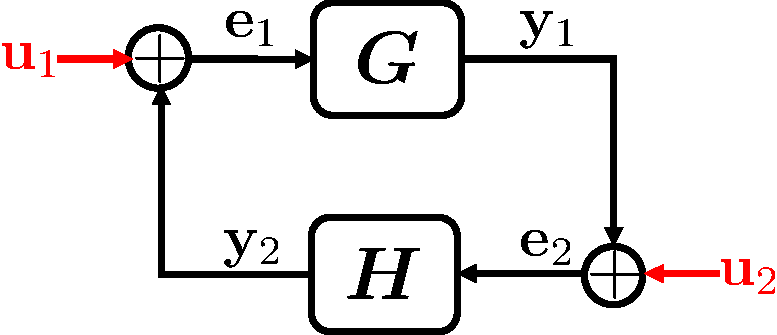
\includegraphics[width=.45\columnwidth]{well-posed}
\caption{A feedback interconnection between systems $\mathbf{G}$ and $\mathbf{H}$.}
\label{fig:well-posed}
\end{figure}

The rest of the paper is structured as follows: in \S \ref{sec:notation}, we introduce notation and basic definitions of stability and well-posedness.  In \S \ref{sec:operator}, we review the SLS parameterization for finite-dimensional LTI systems, and generalize it to a richer class of systems with dynamics described by bounded linear operators.  In \S \ref{sec:robust-perf}, we consider a robust version of the generalized SLS parameterization derived in \S \ref{sec:robust-perf}, and provide necessary and sufficient conditions for robust performance in terms of \emph{convex} constraints on the system responses.  In \S \ref{sec:extensions}, we highlight how these convex constraints can naturally be integrated with structural constraints on the system responses, such as delay, sparsity, and locality constraints, while still preserving the necessity and sufficiency of the identified conditions.  In \S \ref{sec:experiments}, we demonstrate the usefulness of our results on numerical examples, and we end  with conclusions and discussions of future work in \S \ref{sec:conclusion}.